\documentclass[a4paper, 11pt, oneside]{article}

\usepackage[utf8]{inputenc}
\usepackage[T1]{fontenc}
\usepackage[french]{babel}
\usepackage{array}
\usepackage{shortvrb}
\usepackage{listings}
\usepackage[fleqn]{amsmath}
\usepackage{amsfonts}
\usepackage{fullpage}
\usepackage{enumerate}
\usepackage{graphicx}             % import, scale, and rotate graphics
\usepackage{subfigure}            % group figures
\usepackage{alltt}
\usepackage{url}
\usepackage{indentfirst}
\usepackage{eurosym}
\usepackage{listings}
\usepackage{color}
\usepackage[table,xcdraw,dvipsnames]{xcolor} 

% Change le nom par défaut des listing
\renewcommand{\lstlistingname}{Extrait de Code}

% Change la police des titres pour convenir à votre seul lecteur
\usepackage{sectsty}
\allsectionsfont{\sffamily\mdseries\upshape} 
% Idem pour la table des matière.
\usepackage[nottoc,notlof,notlot]{tocbibind} 
\usepackage[titles,subfigure]{tocloft} 
\renewcommand{\cftsecfont}{\rmfamily\mdseries\upshape}
\renewcommand{\cftsecpagefont}{\rmfamily\mdseries\upshape} 

\definecolor{mygray}{rgb}{0.5,0.5,0.5}
\newcommand{\coms}[1]{\textcolor{MidnightBlue}{#1}}

\lstset{
    language=C, % Utilisation du langage C
    commentstyle={\color{MidnightBlue}}, % Couleur des commentaires
    frame=single, % Entoure le code d'un joli cadre
    rulecolor=\color{black}, % Couleur de la ligne qui forme le cadre
    stringstyle=\color{RawSienna}, % Couleur des chaines de caractères
    numbers=left, % Ajoute une numérotation des lignes à gauche
    numbersep=5pt, % Distance entre les numérots de lignes et le code
    numberstyle=\tiny\color{mygray}, % Couleur des numéros de lignes
    basicstyle=\tt\footnotesize, 
    tabsize=3, % Largeur des tabulations par défaut
    keywordstyle=\tt\bf\footnotesize\color{Sepia}, % Style des mots-clés
    extendedchars=true, 
    captionpos=b, % sets the caption-position to bottom
    texcl=true, % Commentaires sur une ligne interprétés en Latex
    showstringspaces=false, % Ne montre pas les espace dans les chaines de caractères
    escapeinside={(>}{<)}, % Permet de mettre du latex entre des <( et )>.
    inputencoding=utf8,
    literate=
  {á}{{\'a}}1 {é}{{\'e}}1 {í}{{\'i}}1 {ó}{{\'o}}1 {ú}{{\'u}}1
  {Á}{{\'A}}1 {É}{{\'E}}1 {Í}{{\'I}}1 {Ó}{{\'O}}1 {Ú}{{\'U}}1
  {à}{{\`a}}1 {è}{{\`e}}1 {ì}{{\`i}}1 {ò}{{\`o}}1 {ù}{{\`u}}1
  {À}{{\`A}}1 {È}{{\`E}}1 {Ì}{{\`I}}1 {Ò}{{\`O}}1 {Ù}{{\`U}}1
  {ä}{{\"a}}1 {ë}{{\"e}}1 {ï}{{\"i}}1 {ö}{{\"o}}1 {ü}{{\"u}}1
  {Ä}{{\"A}}1 {Ë}{{\"E}}1 {Ï}{{\"I}}1 {Ö}{{\"O}}1 {Ü}{{\"U}}1
  {â}{{\^a}}1 {ê}{{\^e}}1 {î}{{\^i}}1 {ô}{{\^o}}1 {û}{{\^u}}1
  {Â}{{\^A}}1 {Ê}{{\^E}}1 {Î}{{\^I}}1 {Ô}{{\^O}}1 {Û}{{\^U}}1
  {œ}{{\oe}}1 {Œ}{{\OE}}1 {æ}{{\ae}}1 {Æ}{{\AE}}1 {ß}{{\ss}}1
  {ű}{{\H{u}}}1 {Ű}{{\H{U}}}1 {ő}{{\H{o}}}1 {Ő}{{\H{O}}}1
  {ç}{{\c c}}1 {Ç}{{\c C}}1 {ø}{{\o}}1 {å}{{\r a}}1 {Å}{{\r A}}1
  {€}{{\euro}}1 {£}{{\pounds}}1 {«}{{\guillemotleft}}1
  {»}{{\guillemotright}}1 {ñ}{{\~n}}1 {Ñ}{{\~N}}1 {¿}{{?`}}1
}
\newcommand{\tablemat}{~}

%%%%%%%%%%%%%%%%% TITRE %%%%%%%%%%%%%%%%
% Complétez et décommentez les définitions de macros suivantes :
\newcommand{\intitule}{Multiplicité du maximum}
\newcommand{\GrNbr}{S190632}
\newcommand{\PrenomUN}{Luca}
\newcommand{\NomUN}{Matagne}
% \newcommand{\PrenomDEUX}{Octave}
% \newcommand{\NomDEUX}{Urbain}
% Décommentez ceci si vous voulez une table des matières :
\renewcommand{\tablemat}{\tableofcontents}

%%%%%%%% ZONE PROTÉGÉE : MODIFIEZ UNE DES DIX PROCHAINES %%%%%%%%
%%%%%%%%            LIGNES POUR PERDRE 2 PTS.            %%%%%%%%
\title{INFO0947: \intitule}
\author{Groupe \GrNbr : \PrenomUN~\textsc{\NomUN}, \PrenomDEUX~\textsc{\NomDEUX}}
\date{}
\begin{document}
\maketitle
\newpage
\tablemat
\newpage
%%%%%%%%%%%%%%%%%%%% FIN DE LA ZONE PROTÉGÉE %%%%%%%%%%%%%%%%%%%%

%%%%%%%%%%%%%%%% RAPPORT %%%%%%%%%%%%%%%
% Écrivez votre rapport ci-dessous.

\section{Formalisation du problème}





\section{Spécification formelle}

Il est importatn de déterminer la précondition et la postcondition de notre problèmes, qui seront le point de départ (pré) et d'arrivée (post)  de notre raisonnement constructif.

Voici ces conditions:

\begin{itemize}

\item Précondition

\begin{center}
    
 N > 0 $\land$ T[N]!= NULL    

\end{center}

\item Postcondition

\begin{center}
    
 max = max(T[N]) $\land$ multiplicite()=nombre d'occurence du maximum 

\end{center}

\end{itemize}


\section{Découpe en sous problèmes}

Etant donné que le problème s'articule autour d'une seule boucle principale et que le fait de diviser le problème en deux SP qui seraient :

1) Recherche du maximum

2) Comptage du nombre d'occurence du maximum

amènerait a une mécompréhension (une telle découpe laisserait croire qu'il nous faut deux boucles).
Je décide de ne pas diviser le problème principal en différents SP.




\section{Invariant graphique et formel de la boucle}

\begin{center}

Voici l'invariant graphique de ma boucle 'while':

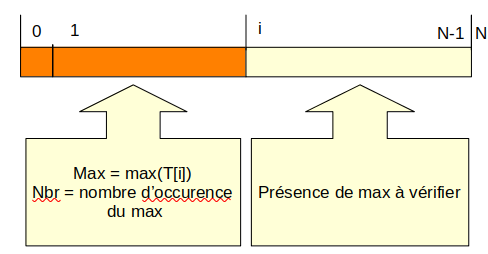
\includegraphics[width=0.70\textwidth]{gliprojet1.png}

\end{center}

Et voici l'invariant formel qui en découle:

\begin{center}

N>0 $\land$ T[N] != NULL $\land$ 1$\leq$i$\leq$N $\land$ max = max(T[i]) $\land$ nbr$\geq$1

\end{center}

\section{Approche constructive}

Dans cette section se trouve l'approche constructive qui m'a permis de construire mon fichier "multiplicite.c" 
\subsection{Code d'innitialisation de la boucle}

\begin{lstlisting}[caption={Code d'innitialisation de la boucle}]

//{N>0 $\land$ T[N] != NULL}
int i = 1;
//{N>0 $\land$ T[N] != NULL $\land$ 1$\leq$i$\leq$N}
int nbr = 1;
//{N>0 $\land$ T[N] != NULL $\land$ 1$\leq$i$\leq$N $\land$ nbr$\geq$1}
int max = T[i];
//N>0 $\land$ T[N] != NULL $\land$ 1$\leq$i$\leq$N $\land$ max = max(T[i]) $\land$ nbr$\geq$1

\end{lstlisting}

\subsection{Corps de la boucle}

\begin{lstlisting}[caption={Corps de la boucle}]

//N>0 $\land$ T[N] != NULL $\land$ 1$\leq$i$\leq$N $\land$ max = max(T[i]) $\land$ nbr$\geq$1
while(i<N);
//N>0 $\land$ T[N] != NULL $\land$ 1$\leq$i$\leq$N $\land$ max = max(T[i]) $\land$ nbr$\geq$1 $\land$ i<N
if(T[i] > max){
//N>0 $\land$ T[N] != NULL $\land$ 1$\leq$i<N $\land$ max = max(T[i]) $\land$ nbr$\geq$1 $\land$ i<N $\land$ T[i]>max
max = T[i];
nbr = 1;
}
//N>0 $\land$ T[N] != NULL $\land$ 1$\leq$i<N $\land$ max = max(T[i]) $\land$ nbr$\geq$1
else if(T[i]==max){
//N>0 $\land$ T[N] != NULL $\land$ 1$\leq$i<N $\land$ max = max(T[i]) $\land$ nbr$\geq$1 $\land$ T[i]=max
nbr++;
}
//N>0 $\land$ T[N] != NULL $\land$ 1$\leq$i<N $\land$ max = max(T[i]) $\land$ nbr$\geq$1
i++;
//N>0 $\land$ T[N] != NULL $\land$ 1$\leq$i$\leq$N $\land$ max = max(T[i]) $\land$ nbr$\geq$1

\end{lstlisting}


\subsection{Code de terminaison de la boucle}

\begin{lstlisting}[caption={Code de terminaison de la boucle}]

//N>0 $\land$ T[N] != NULL $\land$ max = max(T[i]) $\land$ nbr$\geq$1 $\land$ i=N
//N>0 $\land$ T[N] != NULL $\land$ max = max(T[N]) $\land$ nbr$\geq$1
return nbr;
//N>0 $\land$ T[N] != NULL $\land$ max = max(T[N]) $\land$ multiplicite = nombre d'occurence du maximum

\end{lstlisting}


\section{Code complet}


\subsection{main.c}

\begin{lstlisting}[caption={Main.c}]
#include <stdio.h>
#include "multiplicite.h"


int main(){

   int T[8] = {13, -1, 16, 9, -12, 2, 4, 16};
   int max;

   multiplicite(T, 8, &max);

   printf("%d - %d\n", multiplicite(T, 8, &max), max);
}//fin main
\end{lstlisting}


\subsection{multiplicite.c}

\begin{lstlisting}[caption={multiplicite.c}]
#include "multiplicite.h"

int multiplicite(int *T, const int N,  int *max){
   
    int i = 1;
    int nbr = 1;
    *max = T[0]; // le minimum pour un entier 

    while(i<N){

        if(T[i]> *max){

            *max = T[i];
            nbr = 1;

        }else if(T[i]== *max){

            nbr++;

        }

        i++;

    }

   return nbr;

}
\end{lstlisting}


\subsection{multiplicite.h}

\begin{lstlisting}[caption={multiplicite.h}]
#ifndef __MULTIPLICITE_T__
#define __MULTIPLICITE_T__

/**
 * multiplicite
 * 
 * @pre : N > 0 $\land$ T[N]!= NULL
 * 
 * @post : max = max(T[N]) 
 * 
 * @return : multiplicite()=nombre d'occurence du maximum 
 * 
**/

int multiplicite(int *T, const int N,  int *max);

#endif
\end{lstlisting}


\subsection{makefile}

\begin{lstlisting}[caption={makefile}]
CC=gcc
LD=gcc
CFLAGS=--std=c99 --pedantic -Wall -W -Wmissing-prototypes
LDFLAGS=
EXEC=output

all:$(EXEC)

output: main.o multiplicite.o
	$(LD) -o output main.o multiplicite.o $(LDFLAGS)

main.o: main.c
	$(CC) -c main.c -o main.o $(CFLAGS)

multiplicite.o: multiplicite.c multiplicite.h
	$(CC) -c multiplicite.c -o multiplicite.o $(CFLAGS)
\end{lstlisting}





\end{document}

